%%%%%%%%%%%%%%%%%%%%%%%%%%%%%%%%%%%%%%%%%%%%%%%%%%%%%%%%%%%%%%%%%%%%%%%%%%%%%%%%
%% 数学 %%%%%%%%%%%%%%%%%%%%%%%%%%%%%%%%%%%%%%%%%%%%%%%%%%%%%%%%%%%%%%%%%%%%%%%%
%%%%%%%%%%%%%%%%%%%%%%%%%%%%%%%%%%%%%%%%%%%%%%%%%%%%%%%%%%%%%%%%%%%%%%%%%%%%%%%%
%%%%%%%%%%%%%%%%%%%%%%%%%%%%%%%%%%%%%%%%%%%%%%%%%%%%%%%%%%%%%%%%%%%%%%%%%%%%%%%%
\part{数学}

%%%%%%%%%%%%%%%%%%%%%%%%%%%%%%%%%%%%%%%%%%%%%%%%%%%%%%%%%%%%%%%%%%%%%%%%%%%%%%%%
%% 统计和概率学 %%%%%%%%%%%%%%%%%%%%%%%%%%%%%%%%%%%%%%%%%%%%%%%%%%%%%%%%%%%%%%%%
%%%%%%%%%%%%%%%%%%%%%%%%%%%%%%%%%%%%%%%%%%%%%%%%%%%%%%%%%%%%%%%%%%%%%%%%%%%%%%%%
\chapter{统计和概率学}

%%%%%%%%%%%%%%%%%%%%%%%%%%%%%%%%%%%%%%%%%%%%%%%%%%%%%%%%%%%%%%%%%%%%%%%%%%%%%%%%
%% 随机变量 %%%%%%%%%%%%%%%%%%%%%%%%%%%%%%%%%%%%%%%%%%%%%%%%%%%%%%%%%%%%%%%%%%%%
\section{随机变量}

随机变量是一个定义在样本空间中的实值函数。比如我们令 $Y$ 表示投掷三枚硬币正面朝上的次数,那么 $Y$ 就是一个随机变量,有
\begin{align*}
    P\left\{Y = 0\right\} & = 1 / 8 \\
    P\left\{Y = 1\right\} & = 3 / 8 \\
    P\left\{Y = 2\right\} & = 3 / 8 \\
    P\left\{Y = 3\right\} & = 1 / 8
\end{align*}

对于随机变量 $X$,我们定义它的累积分布函数(简称分布函数)为
\[
    F(x) = P\left\{ X \le x \right\} \quad -\infty < x < \infty
\]

根据随机变量的取值情况,我们可以将随机变量分为离散型随机变量和连续型随机变量。

我们可以使用概率分布列来表示离散型随机变量。随机变量 $X$ 的概率分布列 $p(a)$ 被定义为
\[
    p(a) = P\left\{ X = a \right\}
\]

如果 $X$ 的可能取值构成集合 $\{x_1, x_2, \ldots\}$,那么 $\sum_{i = 1}^\infty p(x_i) = 1$。而分布函数因此可以表示为
\[
    F(a) = \sum_{x \le a} p(x)
\]

因为是离散的,所以对应的分布函数 $F(a)$ 是一个阶梯函数,在 $x_i$ 处有跳跃,跃值为 $p(x_i)$。

%%%%%%%%%%%%%%%%%%%%%%%%%%%%%%%%%%%%%%%%%%%%%%%%%%%%%%%%%%%%%%%%%%%%%%%%%%%%%%%%
%% 期望 %%%%%%%%%%%%%%%%%%%%%%%%%%%%%%%%%%%%%%%%%%%%%%%%%%%%%%%%%%%%%%%%%%%%%%%%
\section{期望}

%% 离散型随机变量的期望 %%%%%%%%%%%%%%%%%%%%%%%%%%%%%%%%%%%%%%%%%%%%%%%%%%%%%%%%
\subsection{离散型随机变量的期望}

对于离散型随机变量 $X$,它的期望记为 $E[X]$,定义为
\[
    E[X] = \sum_{x:\ p(x) > 0} x p(x)
\]

即 $X$ 所有可能取值的一个加权平均。即我们对 $X$ 进行若干次实验后,得到的值的平均值会趋向于 $E[X]$。

进一步地,我们能计算出离散型随机变量的函数 $g(X)$ 的期望。我们可以按照离散型随机变量的期望的定义来计算,即我们先计算出 $g(X)$ 的概率分布列,然后再计算出它的期望。

\begin{exampleBox}
    比如对于离散型随机变量 $X$ 有概率分布列 $p_X( \cdot )$ 如下

    \[
        p_X(-1) = 0.2 \qquad p_X(0) = 0.5 \qquad p_X(1) = 0.3
    \]

    那么 $X$ 的函数 $g(X) = X^2$ 有概率分布列 $p_{g(X)}( \cdot )$ 如下

    \[
        p_{g(X)}(0) = 0.5 \qquad p_{g(X)}(1) = 0.5
    \]

    容易得到 $E[X] = 0.1$,而 $E[X^2] = 0.5$。从这里我们就可以看出来,$(E[X])^2 \ne E[X^2]$。
\end{exampleBox}

我们可以更规范地说,对于 $E[g(X)]$,我们有
\[
    E[g(X)] = \sum_{i} g(x_i) p(x_i)
\]

%% 随机变量和的期望 %%%%%%%%%%%%%%%%%%%%%%%%%%%%%%%%%%%%%%%%%%%%%%%%%%%%%%%%%%%%
\subsection{随机变量和的期望}

不妨假设样本空间 $S$ 是一个有限的或者可数无限的集合。
给定一个随机变量 $X$,则当 $s \in S$ 时,令 $X(s)$ 表示此时随机变量 $X$ 的取值,而 $Y$ 同理,即 $Z = X + Y$ 同样是随机变量,而且 $Z(s) = X(s) + Y(s)$ 成立。

举例来说,我们假设随机试验由抛掷 5 次硬币组成,那么这里的一个样本 $s \in S$ 可能为 $(h, t, h, t, h)$。
而 $X$ 表示前三次抛掷中正面朝上的次数,那么 $X(s) = 2$,而 $Y$ 表示后两次抛掷中正面朝上的次数,那么 $Y(s) = 1$,而 $Z(s) = X(s) + Y(s) = 3$。

令 $p(s) = P(\{ s \})$,因为任意事件 $A$ 可以写为有限个或可数无限个互不相容的事件 $s$ 的和,则
\[
    P(A) = \sum_{s \in A} p(s)
\]

假设随机变量 $X$ 的不同取值为 $x_i ( i \ge 1 )$。对于每一个 $i$,令 $S_i$ 表示 $X$ 等于 $x_i$ 时的事件,即 $S_i = \{ s: X(s) = x_i \}$,那么
\begin{align*}
    E[X] & = \sum_{i} x_i P\{ X = x_i \} = \sum_{i} x_i P(S_i) = \sum_{i} x_i \sum_{s \in S_i} p(s) = \sum_{i} \sum_{s \in S_i} x_i p(s) \\
         & = \sum_i \sum_{s \in S_i} X(s) p(s) = \sum_{s \in S} X(s) p(s)
\end{align*}
即 $E[X]$ 有
\[
    E[X] = \sum_{s \in S} X(s) p(s)
\]

对于随机变量 $X_1, X_2, \cdots, X_n$,记 $Z = \sum_{i = 1}^n X_i$,那么有为
\begin{align*}
    E[Z] & = \sum_{s \in S} Z(s) p(s) = \sum_{s \in S} \left( X_1(s) + X_2(s) + \cdots + X_n(s) \right) p(s) \\
         & = \sum_{s \in S} X_1(s) p(s) + \sum_{s \in S} X_2(s) p(s) + \cdots + \sum_{s \in S} X_n(s) p(s) \\
         & = E[X_1] + E[X_2] + \cdots + E[X_n]
\end{align*}
即,随机变量的和的期望即为随机变量的期望的和。

%%%%%%%%%%%%%%%%%%%%%%%%%%%%%%%%%%%%%%%%%%%%%%%%%%%%%%%%%%%%%%%%%%%%%%%%%%%%%%%%
%% 期望 %%%%%%%%%%%%%%%%%%%%%%%%%%%%%%%%%%%%%%%%%%%%%%%%%%%%%%%%%%%%%%%%%%%%%%%%
\section{方差和标准差}

对于随机变量 $X$ 而言,我们定义方差 $\textrm{Var}(X)$ 为
\[
    \textrm{Var}(X) = E\left[ (X - E[X])^2 \right]
\]

但是我们可以对其进行推导,从而得到一个等价的,但是很有意思的表达,即
\[
    \textrm{Var}(X) = E[X^2] - (E[X])^2
\]
这个推导是很简单的。我们还很容易能够发现,根据方差的定义,方差一定大于等于 $0$,所以能说,对于随机变量,它的平方的期望一定大于等于期望的平方。

对于 $X$ 而言,我们定义它的标准差为
\[
    \textrm{SD}(X) = \sqrt{\textrm{Var}(X)}
\]

%%%%%%%%%%%%%%%%%%%%%%%%%%%%%%%%%%%%%%%%%%%%%%%%%%%%%%%%%%%%%%%%%%%%%%%%%%%%%%%%
%% 离散型随机变量 %%%%%%%%%%%%%%%%%%%%%%%%%%%%%%%%%%%%%%%%%%%%%%%%%%%%%%%%%%%%%%
\section{离散型随机变量}

%% 伯努利随机变量和二项随机变量 %%%%%%%%%%%%%%%%%%%%%%%%%%%%%%%%%%%%%%%%%%%%%%%%
\subsection{伯努利随机变量和二项随机变量}

对于随机变量 $X$,如果它的分布列满足
\begin{align*}
    p(0) & = P\left\{ X = 0 \right\} = 1 - p \\
    p(1) & = P\left\{ X = 1 \right\} = p
\end{align*}
其中 $p \in (0, 1)$,那么我们说 $X$ 为伯努利随机变量。

我们假设我们做了 $n$ 次实验,其中每一次实验结果都可以看成一个独立的伯努利随机变量(实验成功,我们则将其记为 $1$,那么实验成功的概率为 $p(1) = p$),那么最后成功的次数也是一个随机变量,我们记它为参数为 $(n, p)$ 的二项随机变量 $X$,它的分布列为
\[
    p(i) = {n \choose i} p^i (1 - p)^{n - i} \qquad i = 0, 1, \cdots, n
\]

伯努利随机变量是参数为 $(1, p)$ 的特殊二项随机变量。

对于二项随机变量 $X$ 而言,不让认为它的参数为 $(n, p)$,那么有期望为
\begin{align*}
    E[X] & = \sum_{i = 0}^{n} i p(i) = \sum_{i = 1}^{n} i p(i) \\
         & = \sum_{i = 1}^{n} i {n \choose i} p^i (1 - p)^{n - i} \\
         & = \sum_{i = 1}^{n} i {n! \over i! (n - i)!} p^i (1 - p)^{n - i} \\
         & = np \sum_{i = 1}^{n} {(n - 1)! \over (i - 1)! \left[(n - 1) - (i - 1)\right]!} p^{i - 1} (1 - p)^{(n - 1) - (i - 1)} \\
         & = np \sum_{j = 0}^{m} {m! \over j! (m - j)!} p^j (1 - p)^{m - j} \\
         & = np
\end{align*}
这里我们知道 $\sum_{j = 0}^{m} {m! \over j! (m - j)!} p^j (1 - p)^{m - j} = 1$,所以能够知道对于参数为 $(n, p)$ 的二项随机变量 $X$ 而言,$E[X] = np$。

我们可以进一步地解随机变量的次方对应的随机变量 $X^k$ 的期望,有
\begin{align*}
    E[X^k] & = \sum_{i = 1}^{n} i^k {n \choose i} p^i (1 - p)^{n - i} \\
           & = \sum_{i = 1}^{n} i^{k - 1} n {n - 1 \choose i - 1} p^i (1 - p)^{n - i} \qquad \textrm{这里有 $i {n \choose i} = n {n - 1 \choose i - 1}$} \\
           & = np \sum_{i = 1}^{n} i^{k - 1} {n - 1 \choose i - 1} p^{i - 1} (1 - p)^{n - i} \\
           & = np \sum_{j = 0}^{n - 1} (j + 1)^{k - 1} {n - 1 \choose j} p^j (1 - p)^{(n - 1) - j} \\
           & = np E[(Y + 1)^{k - 1}]
\end{align*}
其中 $Y$ 为一个二项随机变量,它的参数为 $(n - 1, p)$。那么有
\begin{align*}
    E[X^2] & = np E[Y + 1] \\
           & = np [(n - 1)p + 1]
\end{align*}
带入到方差的公式中,有
\begin{align*}
    \textrm{Var}(X) = E[X^2] - (E[X])^2 = np [(n - 1)p + 1] - (np)^2 = np (1 - p)
\end{align*}

给出一个重要结论,对于参数为 $(n, p)$ 的二项随机变量 $X$,有
\begin{center}
    \fbox{$ E[X] = np \qquad \textrm{Var}(X) = np (1 - p) $}
\end{center}

此外,我们需要意识到,如果 $X$ 是参数 $(n, p)$ 对应的二项随机变量,那么对于 $k$ 从 $0$ 到 $n$,其 $P\{ X = k \}$ 会先单调递增,然后再单调递减。当 $k$ 为
\[
    \left\lfloor (n + 1) p \right\rfloor
\]
时,$P\{X = k\}$ 取得最大值。

%% 柏松随机变量 %%%%%%%%%%%%%%%%%%%%%%%%%%%%%%%%%%%%%%%%%%%%%%%%%%%%%%%%%%%%%%%%
\subsection{泊松随机变量}

对于随机变量 $X$,如果满足
\[
    p(i) = P\{X = i\} = e^{-\lambda} {\lambda^i \over i!} \qquad i = 0, 1, 2, \ldots
\]
那么我们说 $X$ 是服从参数 $\lambda$ 的泊松随机变量。当 $n$ 足够大,然后 $p$ 又足够小使得 $np$ 保持适当的大小的时候,那么参数为 $(n, p)$ 的二项随机变量可以近似地看为服从 $\lambda = np$ 的泊松随机变量(反过来也成立)。也就是说,对于满足这个条件的二项随机变量 $X$ 有
\begin{align*}
    P\{X = i\} & = {n \choose i} p^i (1 - p)^{n - i} = {n! \over i! (n - i)!} \left( {\lambda \over n} \right)^i \left( 1 - {\lambda \over n} \right)^{n - i} \\
               & = {n (n - 1) \cdots (n - i + 1) \over i!} {\lambda^i \over n^i} {(1 - \lambda / n)^n \over (1 - \lambda / n)^i}
\end{align*}
对于充分大的 $n$ 和适当的 $\lambda$,有\footnote{书中没有指出来,但是我看这第三个表达式的含义恐怕需要 $i$ 也不能太大?似乎因为 $np$ 本身保持适当的值,所以导致 $i$ 取 $np$ 附近的值时,$p(i)$ 的值才会比较大的样子,似乎 $i$ 过大的情况下,$p(i)$ 就会约等于 $0$ 了。}
\[
    \left(1 - {\lambda \over n}\right)^n \approx e^{-\lambda}, \qquad n (n - 1) \cdots (n - i + 1) \approx n^i, \qquad \left(1 - {\lambda \over n}\right)^i \approx 1
\]
那么有
\[
    P\{X = i\} = {\lambda^i \over i!} e^{-\lambda}
\]

举例来说,某页印刷错的字母个数 $X$ 即可以视为泊松随机变量。每个字母印刷错误的概率很小,为 $p$,该页的字母个数为 $n$,那么 $X$ 的参数 $\lambda$ 满足 $\lambda = np$。

我们知道,对于二项随机变量而言,期望和方差分别为 $np$ 和 $np(1 - p)$。因为泊松随机变量可以视为特殊情况下的二项随机变量,所以泊松分布的期望和方差可以带入得到 $\lambda$ 和 $\lambda$(因为 $p$ 很小,所以我们认为 $1 - p$ 可以视为 $1$)。

%% 几何随机变量 %%%%%%%%%%%%%%%%%%%%%%%%%%%%%%%%%%%%%%%%%%%%%%%%%%%%%%%%%%%%%%%%
\subsection{几何随机变量}

考虑独立重复实验中,反复实验,直到实验成功的实验总次数 $X$ 为一个随机变量,那么有
\[
    P\{ X = n\} = (1 - p)^{n - 1} p \qquad n = 1, 2, \cdots
\]
那么我们说 $X$ 是服从参数 $p$ 的几何随机变量。几何随机变量的期望为
\[
    E[X] = {1 \over p}
\]
方差为
\[
    \textrm{Var}(X) = {1 - p \over p^2}
\]

%% 负二项随机变量 %%%%%%%%%%%%%%%%%%%%%%%%%%%%%%%%%%%%%%%%%%%%%%%%%%%%%%%%%%%%%%
\subsection{负二项随机变量}

负二项随机变量是几何随机变量的一个延伸。考虑独立重复实验中,反复实验,直到实验成功 $r$ 次的实验总次数 $X$ 为一个随机变量,那么有
\[
    P\{ X = n \} = \left( { n - 1 \over r - 1 } \right) (1 - p)^{n - r} p^r
\]
我们称 $X$ 是服从参数 $(r, p)$ 的负二项随机变量。

负二项随机变量的期望为
\[
    E[X] = {r \over p}
\]
方差为
\[
    \textrm{Var}(X) = {r(1 - p) \over p^2}
\]

%% 超几何随机变量 %%%%%%%%%%%%%%%%%%%%%%%%%%%%%%%%%%%%%%%%%%%%%%%%%%%%%%%%%%%%%%
\subsection{超几何随机变量}

考虑一个坛子中有 $N$ 个球,其中 $m$ 个白球,$N - m$ 个黑球,从中随机无放回地抽取 $n$ 个球,设随机变量 $X$ 为抽到的白球个数,那么我们说 $X$ 是服从参数 $(n, N, m)$ 的超几何随机变量。那么有
\[
    P\{ X = i \} = {{m \choose i} {N - m \choose n - i} \over {N \choose n}} \qquad i = 0, 1, \cdots, n
\]
这个的表达式是直观的。注,我们定义了 $k < 0$ 或者 $r < k$ 时 $r \choose k$ 等于 $0$。

当 $N$ 和 $m$ 相对 $n$ 而言很大的时候,我们可以认为这个时候是否放回对于结果来说是没有影响的。也就是说,超几何随机变量可以近似地看成二项随机变量。

超几何随机变量的期望为
\[
    E[X] = {nm \over N}
\]
方差为
\[
    \textrm{Var}(X) = {nm \over N}\left[ {(n - 1)(m - 1) \over N - 1} + 1 - {nm \over N} \right]
\]
如果令 $p = m / N$,那么有为
\[
    E[X] = np \qquad \textrm{Var}(X) = np(1 - p){1- {n - 1 \over N - 1}}
\]

%% Zeta 随机变量 %%%%%%%%%%%%%%%%%%%%%%%%%%%%%%%%%%%%%%%%%%%%%%%%%%%%%%%%%%%%%%%
\subsection[zeta 分布]{$\zeta$ 分布}

如果一个随机变量有如下的分布列:
\[
    P\{X = k\} = {C \over k^{\alpha + 1}} \qquad k = 1, 2, \cdots
\]
其中 $\alpha > 0$ 为参数,则称该随机变量为服从 $\zeta$ 分布(或者说 Zipf 分布)。而因为概率之和必然等于 1,所以有:
\[
    C = \left[ \sum_{k = 1}^\infty \left( {1 \over k} \right)^{\alpha + 1} \right]^{-1}
\]

%% 概率密度函数 %%%%%%%%%%%%%%%%%%%%%%%%%%%%%%%%%%%%%%%%%%%%%%%%%%%%%%%%%%%%%%%%
\subsection{概率密度函数}

对于随机变量 $X$,我们说它的概率密度函数 $f_X(x)$ 可以用来描述 $X$ 随机变量能够取某个值的概率大小的函数。也就是说,对于 $\forall -\infty < a < b < \infty$,我们有

$$
P\left[ a < X < b \right] = \int_{a}^{b} f_X(x) \dif{x}
$$

即 $X$ 的取值在 $(a, b)$ 之间的概率正好为概率密度函数在这个区间的积分。

%%%%%%%%%%%%%%%%%%%%%%%%%%%%%%%%%%%%%%%%%%%%%%%%%%%%%%%%%%%%%%%%%%%%%%%%%%%%%%%%
%% 协方差 %%%%%%%%%%%%%%%%%%%%%%%%%%%%%%%%%%%%%%%%%%%%%%%%%%%%%%%%%%%%%%%%%%%%%%
\section{协方差}

我们使用协方差来描述随机变量之间的相关程度。我们定义 $X$ 和 $Y$ 这两个随机变量的协方差为

$$
\textrm{cov}(X, Y) = E\left[ ( X - E[X] ) ( Y - E[Y] ) \right]
$$

如果我们说两个随机变量 $X$ 和 $Y$ 正相关的时候,
那么当 $X$ 大于 $E[X]$ 的时候,一般来说,$Y$ 也大概率大于 $E[Y]$,反之亦然。
带入式子可以看出 $\textrm{cov}(X, Y)$ 是大于 $0$ 的。
所以我们可以反过来用协方差来量化地定义两个随机变量之间的相关性。

%%%%%%%%%%%%%%%%%%%%%%%%%%%%%%%%%%%%%%%%%%%%%%%%%%%%%%%%%%%%%%%%%%%%%%%%%%%%%%%%
%% 连续型随机变量 %%%%%%%%%%%%%%%%%%%%%%%%%%%%%%%%%%%%%%%%%%%%%%%%%%%%%%%%%%%%%%
\section{连续型随机变量}

设 $X$ 为一个随机变量。如果存在一个定义在实数轴上的非负函数 $f$,使得对于任一一个实数集 $B$ 满足
\[
    P\left\{ X \in B \right\} = \int_B f(x) \dif{x}
\]
那么 $X$ 是连续型随机变量。而 $f$ 为随机变量 $X$ 的概率密度函数。而其中 $f$ 一定满足
\[
    1 = P\left\{ X \in (-\infty, +\infty) \right\} = \int_{-\infty}^{+\infty} f(x) \dif{x}
\]

所有关于 $X$ 的概率都可以通过 $f$ 得到,即有
\begin{align*}
    P\left\{ a < X < b \right\} & = \int_a^b f(x) \dif{x} \\
    P\left\{ X = a \right\} & = 0 \\
    P\left\{ X < a \right\} & = P\left\{ X \le a \right\} = F(a) = \int_{-\infty}^a f(x) \dif{x}
\end{align*}

%%%%%%%%%%%%%%%%%%%%%%%%%%%%%%%%%%%%%%%%%%%%%%%%%%%%%%%%%%%%%%%%%%%%%%%%%%%%%%%%
%% 正态分布 %%%%%%%%%%%%%%%%%%%%%%%%%%%%%%%%%%%%%%%%%%%%%%%%%%%%%%%%%%%%%%%%%%%%
\section{正态分布}

我们说一个随机变量 $X$ 服从正态分布,那么我们记为 $X \sim N(\mu, \sigma^2)$。

这里的 $\mu$ 表示期望,$\sigma^2$ 表示方差。正态分布的概率密度函数为:

$$
f(x) = {1 \over \sqrt{2\pi}\sigma} \exp\left(-{(x - \mu)^2 \over 2\sigma^2}\right)
$$

我们将 $X \sim N(0, 1)$ 的随机变量称为标准正态分布。这个时候我们带入有概率密度函数如下:

$$
f(x) = {1 \over \sqrt{2\pi}} \exp\left(-{x^2 \over 2}\right)
$$

另外,对于 $X \sim N(\mu, \sigma^2)$ 而言,我们可以说 $Y = {X - \mu \over \sigma}$ 服从标准正态分布。

在 Rust 中,我们可以通过下面的方式来完成模拟(这里的 \verb|v| 即为一个正态分布的抽样):

\begin{lstlisting}
use rand_distr::{Distribution, Normal};

let normal = Normal::new(0.0, 1.0).unwrap();
let v = normal.sample(&mut rand::rng());
println!("{} is from a N(0, 1) distribution", v);
// 0.8033917292233297 is from a N(0, 1) distribution
\end{lstlisting}

在文档项目中的 \verb|playground| 目录下运行下面的命令即可:

\begin{lstlisting}
cargo run --bin 00_normal
\end{lstlisting}

%%%%%%%%%%%%%%%%%%%%%%%%%%%%%%%%%%%%%%%%%%%%%%%%%%%%%%%%%%%%%%%%%%%%%%%%%%%%%%%%
%% 伊藤引理 %%%%%%%%%%%%%%%%%%%%%%%%%%%%%%%%%%%%%%%%%%%%%%%%%%%%%%%%%%%%%%%%%%%%
\section{伊藤引理}
\label{title:ItosLemma}

[TODO]

%%%%%%%%%%%%%%%%%%%%%%%%%%%%%%%%%%%%%%%%%%%%%%%%%%%%%%%%%%%%%%%%%%%%%%%%%%%%%%%%
%% 标准布朗运动 %%%%%%%%%%%%%%%%%%%%%%%%%%%%%%%%%%%%%%%%%%%%%%%%%%%%%%%%%%%%%%%%
\section{标准布朗运动}

我们这么定义标准布朗运动,对于定义在非负实数(时域)$t$ 上的连续随机过程 $\{B_t, t \ge 0\}$,满足以下条件:

\begin{itemize}
    \item $B(0) = 0$;
    \item 平稳性:对于所有 $0 < s < t$,增量 $B(t) - B(s)$ 符合均值为 $0$,方差为 $t - s$ 的正态分布。
    \item 独立增量:对于所有 $0 \le s < t < u < v$,增量 $B(t) - B(s)$ 和 $B(v) - B(u)$ 是独立的。
\end{itemize}

这个时候我们就说 $B(t)$ 是一个标准布朗运动。

在编程实现中,想要模拟连续的标准布朗运动是不现实且没有必要的,我们可以用离散的方式来模拟。
在 Rust 中,随机数可以通过 \verb|rand| 来生成,但是为了通过正态分布生成随机数,我们还需要使用 \verb|rand_distr|。
我们假设按照单位时间为 1s,那么中国股市的一天的交易时间就一共有 14400 个单位时间(对应 4 个小时)。
我们尝试循环 14400 次,每次都生成单位时间内对应的差 $\Delta B$,并且将其累加到 $B$ 上。
根据标准布朗运动的定义,我们很容易知道 $\Delta B$ 服从一个均值为 0,方差为 1 的标准正态分布(我们定义单位时间的长度就是 $1$)。
然后因为增量都是独立的,所以 $\Delta B$ 的求值和之前的求值无关,这是一个非常优良的特征。这使得下面的代码很容易实现:

\begin{lstlisting}
use rand_distr::{Distribution, Normal};

fn std_brownian_motion(steps: usize) -> Vec<f64> {
    let mut rng = rand::rng();

    let normal = Normal::new(0.0, 1.0).unwrap();
    let mut bm = vec![0.0];

    for _ in 0..steps {
        let v = normal.sample(&mut rng);
        bm.push(bm.last().unwrap() + v);
    }

    bm
}

std_brownian_motion(14400);
\end{lstlisting}

在文档项目中的 \verb|playground| 目录下运行如下命令即可:

\begin{lstlisting}
cargo run --bin 01_std_brownian_motion
\end{lstlisting}

在浏览器中,可以看到标准布朗运动的图像。如图 \ref{fig:stdBrownianMotion} 所示。

\begin{figure}[h]
    \centering
    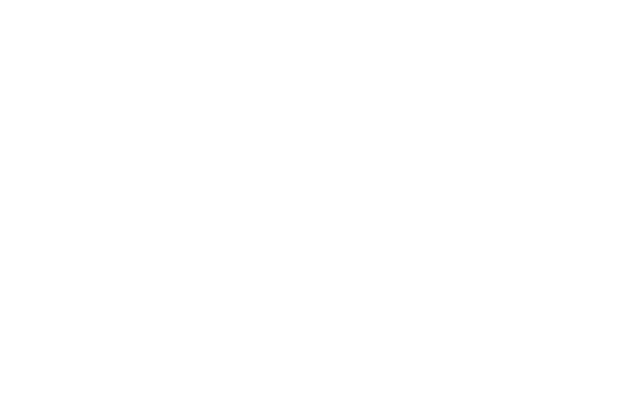
\includegraphics[width=0.8\textwidth]{src/static/00_std_brownian_motion.png}
    \caption{标准布朗运动}
    \label{fig:stdBrownianMotion}
\end{figure}

%%%%%%%%%%%%%%%%%%%%%%%%%%%%%%%%%%%%%%%%%%%%%%%%%%%%%%%%%%%%%%%%%%%%%%%%%%%%%%%%
%% 几何布朗运动 %%%%%%%%%%%%%%%%%%%%%%%%%%%%%%%%%%%%%%%%%%%%%%%%%%%%%%%%%%%%%%%%
\section[几何布朗运动]{几何布朗运动\protect\footnotemark}
\footnotetext{见 \url{https://zhuanlan.zhihu.com/p/38293827}。}

我们可以在标准布朗运动 $B(t)$ 的基础上定义几何布朗运动。在定义之前,我们先定义有漂移的布朗运动 $X(t)$,它有:

$$
\dif{X(t)} = \mu \dif{t} + \sigma \dif{B(t)}
$$

我们知道 $B(t)$ 随机变量在 $t = 1$ 的期望为 $0$,而标准差为 $1$,经过偏移后,$X(t)$ 的期望和方差属性都有所变化。
这里 $\mu$ 被用于表示在单位时间内的期望增长率,而 $\sigma$ 被用于表示单位时间内的标准差。

在量化交易中,我们可以使用这个来描述收益率,而对于股票价格 $S(t)$ 而言,因为有 ${\dif{S(t)} \over S(t)} = \dif{X(t)}$。所以有:

$$
\dif{S(t)} = \mu S(t) \dif{t} + \sigma S(t) \dif{B(t)}
$$

通过伊藤引理 \ref{title:ItosLemma},我们可以得到:

$$
S(t) = S_0 \exp\left(\left(\mu - {\sigma^2 \over 2}\right)t + \sigma B(t)\right)
$$

我们可以使用 Rust 来对齐进行描述:

\begin{lstlisting}
use rand_distr::{Distribution, Normal};

fn geo_brownian_motion(steps: usize, mu: f64, sigma: f64, s0: f64) -> Vec<f64> {
    let mut rng = rand::rng();

    let normal = Normal::new(0.0, 1.0).unwrap();
    let mut bm = vec![s0];

    for _ in 0..steps {
        let z = normal.sample(&mut rng);
        let last_val = bm.last().unwrap();

        let drift = mu - 0.5 * sigma.powi(2);
        let diffusion = sigma * z;
        let new_val = last_val * (drift + diffusion).exp();

        bm.push(new_val);
    }

    bm
}
\end{lstlisting}

在 \verb|playground| 目录下运行如下命令即可:

\begin{lstlisting}
cargo run --bin 02_geo_brownian_motion
\end{lstlisting}

可以在浏览器中看到对应的几何布朗运动的图像。图 \ref{fig:geoBrownianMotion} 展示了几何布朗运动的一个例子。
(在这个图中,我们假定它为一个指数的日内曲线,其中年化收益率为 $8\%$,而一年的方差设置为 $10$)。

\begin{figure}[h]
    \centering
    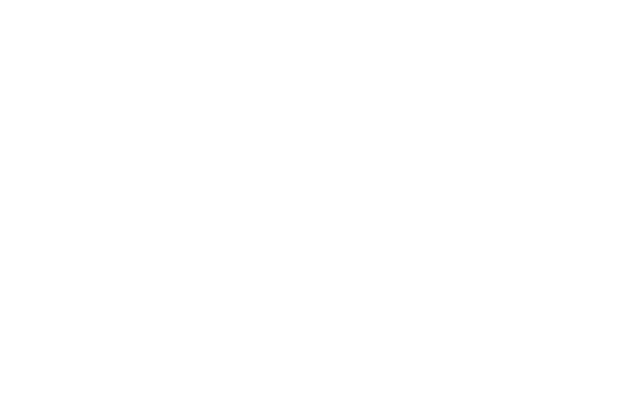
\includegraphics[width=0.8\textwidth]{src/static/01_geo_brownian_motion.png}
    \caption{几何布朗运动}
    \label{fig:geoBrownianMotion}
\end{figure}

